\subsubsection{Testdurchführungsbericht}
Nach der Ausführung der UI-Tests generiert die Testumgebung eine
HTML-Seite, die einen detaillierten Bericht über die Ausführung
der Tests liefert (siehe \autoref{subsubsec:extent}). Dies ermöglicht es
Ihnen, die Ausführung der Tests zu überwachen und mögliche Fehler
zu erkennen.

\begin{figure}[H]
    \centering
    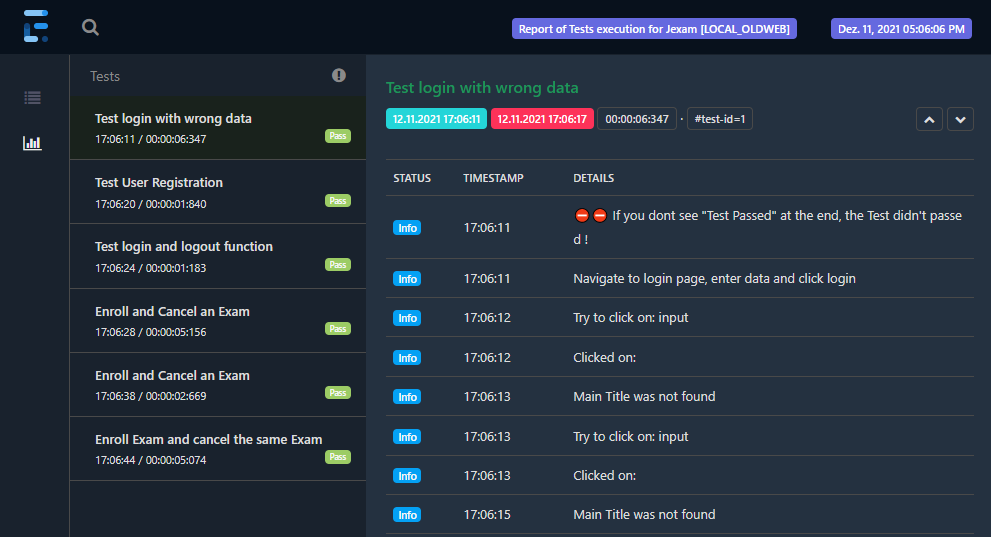
\includegraphics[scale=0.6]{images/ExtentReport}
    \caption{Extent Report HTML Page} \label{fig:ext-rep}
\end{figure}